
%(BEGIN_QUESTION)
% Copyright 2014, Tony R. Kuphaldt, released under the Creative Commons Attribution License (v 1.0)
% This means you may do almost anything with this work of mine, so long as you give me proper credit

Denne induktive nivåreléen for væske produserer 800 volt mellom følesondene når de ikke er i kontakt med væsken, fra en 120 volt AC-kilde:

$$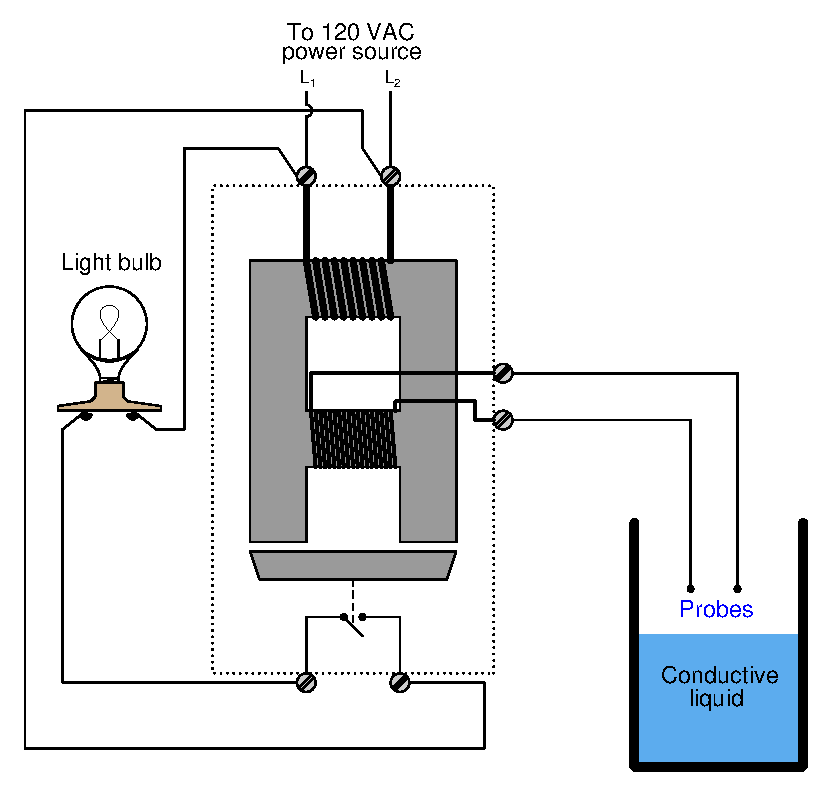
\includegraphics[width=15.5cm]{i00035x01.eps}$$

Forutsatt 200 viklinger i primærviklingen, beregn følgende parametere.  Anta for enkelhets skyld at reléets armatur ennå ikke har "trukket" når væsken først berører sondespissene:

\vskip 10pt

\begin{itemize}
\item{} Antall viklinger i sekundærviklingen = \underbar{\hskip 50pt}
\vskip 10pt 
\item{} Strøm i primærviklingen når væskens $R$ er 20,000 $\Omega$ = \underbar{\hskip 50pt}
\vskip 10pt 
\item{} Strøm i sekundærviklingen når væskens $R$ er 20,000 $\Omega$ = \underbar{\hskip 50pt}
\end{itemize}

\vskip 10pt

Forklar også hvorfor det er viktig å vite at armaturen fortsatt er i "hvile"-posisjon for disse beregningene.

\vfil 

\underbar{file i00035}
\eject
%(END_QUESTION)





%(BEGIN_ANSWER)

Dette er et vurdert spørsmål -- ingen svar eller hint gis!

%(END_ANSWER)





%(BEGIN_NOTES)

Antall viklinger i sekundærviklingen er det som trengs for å gi et forhold (med 200 viklinger i primærviklingen) som kan trinn-opp 120 volt til 800 volt:

$${800 \hbox{ V} \over 120 \hbox{ V} } = {x \over 200 \hbox{ turns}}$$

$$x = 200 \hbox{ turns} \left( 800 \hbox{ V} \over 120 \hbox{ V} \right)$$

$$x = 1333 \hbox{ turns}$$

\vskip 10pt

Strøm i sekundærviklingen bestemmes enkelt ved å bruke Ohms lov, ta 800 volt og dele på motstanden i væsken mellom sondene:

$$I = {V \over R} = {800 \hbox{ V} \over 20000 \> \Omega} = 40 \hbox{ mA}$$

\vskip 10pt

Strøm i primærviklingen må være større enn dette, siden spenningen i primærviklingen er {\it lavere} enn spenningen i sekundærviklingen og effekten ($P = IV$) må være den samme på begge sider av transformatoren.  Vi kan derfor ta spenningsforholdet (800:120) og bruke dette til å beregne primærstrømmen ut fra sekundærstrømmen:

$$I_{primary} = 40 \hbox{ mA} \left( 800 \over 120 \right) = 266.7 \hbox{ mA}$$

\vskip 10pt

Det er viktig å vite at armaturen er i hvileposisjon i disse beregningene fordi når den er det, fungerer den induktive nivåreléen som en enkel step-up-transformator.  Når armaturen trekker inn, dannes en ny magnetisk krets i relékjernen som avleder mye av den magnetiske fluksen fra primærviklingen bort fra sekundærviklingen.  Når det skjer, vil sekundærviklingen gi mye mindre enn 800 volt, og alle strømverdiene blir også redusert!

%INDEX% Switch, level: liquid conductivity

%(END_NOTES)
